Cet outil permet d'appliquer plusieurs algorithmes aux dumps, afin d'aider au repérage de l'information recherchée.

\subsubsection{Similarities \cite {ref-vandeursen}} \label{04-similarities}

Cet algorithme permet de mettre en évidence, dans un groupe de dumps, les chaînes de bits semblables (que nous appellerons \emph{similarités}) ou dissemblables (que nous appellerons \emph{dissimilarités}). Ces chaînes doivent être au même endroit dans chaque dump pour être reconnues.

Dans le cas de deux dumps, les similarités sont représentées par la couleur verte, tandis que les similarités sont représentées par la couleur rouge. Un exemple de similarités est représenté sur la figure \ref{04-1-sim_simple}. Pour faciliter la compréhension, on y a remplacé les bits (de sens à priori inconnu) par des lettres.

\begin{figure}[!h]
  \begin{center}
\small{
  {\tt\center
  {Dump 1 : \color{simColor} \uline{Ce}}{\color{dissimColor} ci es}{\color{simColor}\uline{t} }{\color{dissimColor} un exemple de }{\color{simColor} \uline{similarité}}

  {Dump 2 : \color{simColor} \uline{Ce}}{\color{dissimColor} la me}{\color{simColor}\uline{t} }{\color{dissimColor} en couleur la }{\color{simColor} \uline{similarité}}
  }}
  \end{center}
  \caption{Exemple de similarités}
  \label{04-1-sim_simple}
\end{figure}

Afin d'affiner la recherche, il est possible de spécifier une taille de chaîne minimum, comme l'illustre la figure \ref{04-1-sim_taille_min}.

\begin{figure}[!h]
  \begin{center}
\small{
  {\tt
  {Dump 1 : \color{dissimColor} Ceci est un exemple de }{\color{simColor} \uline{similarité} }{\color{dissimColor} avec une taille minimum de 4}

  {Dump 2 : \color{dissimColor} Cela met en couleur la }{\color{simColor} \uline{similarité} }{\color{dissimColor} faisant plus de 4 caractères}
  }}
  \end{center}
  \caption{Similarités avec une taille de chaîne minimum}
  \label{04-1-sim_taille_min}
\end{figure}


Dans le cas de plusieurs dumps, on dispose de trois couleurs. Le rouge représente les dissimilarités, le vert les similarités concernant le dump visualisé (c'est-à-dire les similarités commune à ce dump et à d'autres), tandis que le bleu correspond aux similarités ne concernant pas le dump visualisé (c'est-à-dire les similarités communes à d'autres dumps).
Ces couleurs ont des nuances : plus le vert ou le bleu sont prononcés, plus il y a de dumps partageant la similarité en question. La figure \ref{04-1-sim_mult} est un exemple de similarités avec 3 dumps.

\begin{figure}[!h]
  \begin{center}
\small{
  {\tt
  {Dump 1 : \color{dissimColor} Encore un}{\color{otherSimColor} \uwave{e au}}{\color{dissimColor} tre }{\color{simColor} \uline{similarité}}{\color{dissimColor} .}

  {Dump 2 : \color{dissimColor} Toujours }{\color{simColor} \uline{plus} }{\color{dissimColor} de }{\color{simColor} \uline{similarité}}{\color{dissimColor} s}

  {Dump 3 : \color{dissimColor} colorées }{\color{simColor} \uline{plus} }{\color{dissimColor} qu'}{\color{otherSimColor} \uwave{auparavant}}{\color{dissimColor} .}
  }}
  \end{center}
  \caption{Similatités entre trois dumps}
  \label{04-1-sim_mult}
\end{figure}

\subsubsection{Dotplot patterns \cite {ref-dotplot}} \label{04-dotplot}

Cet algorithme s'applique à deux dumps et génère un schéma similaire à celui représenté sur la figure \ref{04-1-dotplot}.
Sur ce schéma, on retrouve l'un des dumps en abscisse, et l'autre en ordonnée. Les diagonales représentent des chaînes de bits semblables dans les deux dumps qui, contrairement aux similarités, ne sont pas nécessairement au même emplacement dans chaque dump. Leurs coordonnées représentent leurs positions dans chacun des dumps.
Dans cet exemple, on constate deux diagonales : l'une correspondant à la répétition du mot \texttt{un}, l'autre, plus longue, à celle du mot \texttt{dump}.

\begin{figure}[!h]
  \begin{center}
  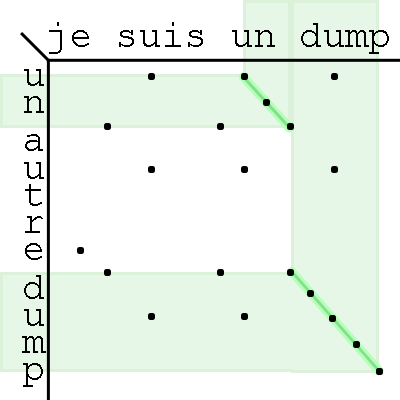
\includegraphics[scale=0.75]{res/04-2-dotplot.png}
  \caption{Un motif obtenu par dotplot}
  \label{04-1-dotplot}
  \end{center}
\end{figure}